\vspace*{-15mm}

\begin{IEEEbiography}[{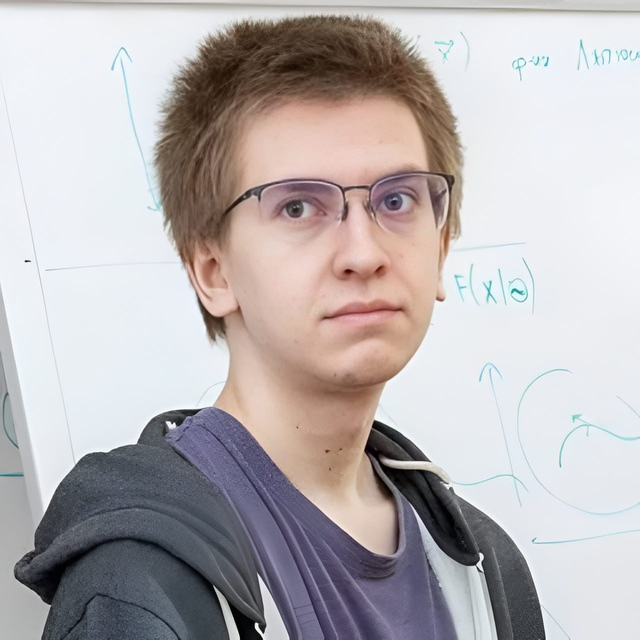
\includegraphics[width=1in,height=1.25in,clip,keepaspectratio]{images/authors/MikhailMenschikov.png}}]{M. Menschikov} received the B.Sc. degree in Software Engineering from Petrozavodsk State University in 2023 and the M.Sc. degree in Machine Learning Engineering from ITMO University in 2025. He is currently a Software Engineer at Skoltech AI Center, where he contributed to a project on developing working memory for LLM agents based on a knowledge graph. His research interests include generative modeling, GraphRAG, LLM-based knowledge graph reasoning, LLM-based knowledge graph construction, multi-agent systems, and dialogue systems.
\end{IEEEbiography}

\vspace*{-15mm}

\begin{IEEEbiography}[{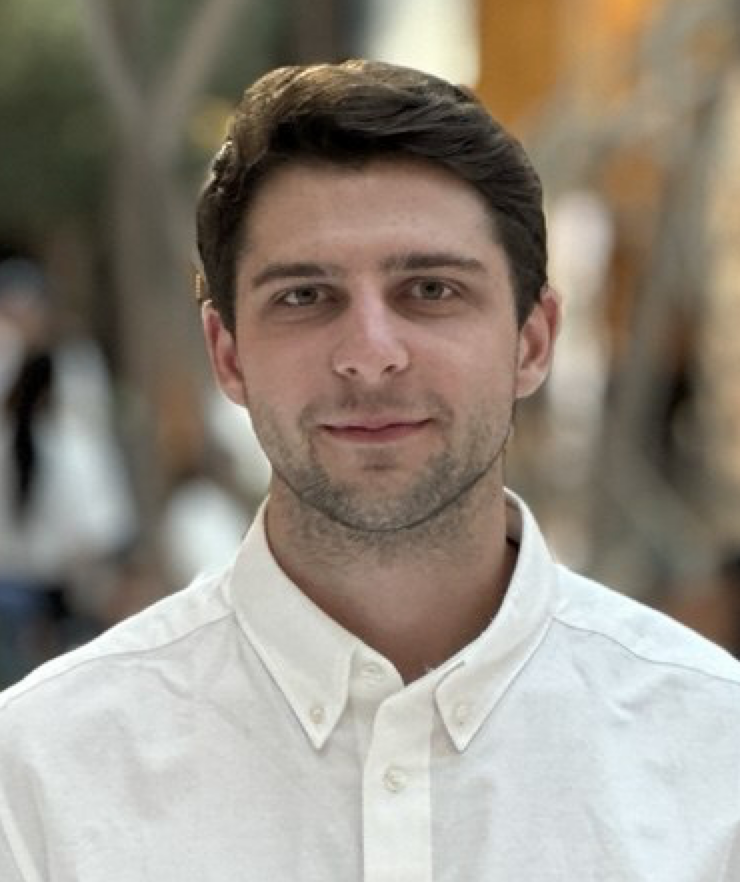
\includegraphics[width=1in,height=1.25in,clip,keepaspectratio]{images/authors/MatveyIskornev.png}}]{M. Iskornev} received the Specialist degree in mathematics from Lomonosov Moscow State University, Faculty of Mechanics and Mathematics, graduating with honors. He is currently an ML Engineer at the Skoltech AI Center, where he works on methods for building knowledge-graph-based memory for LLM agents and improving contextual learning. He has several years of experience developing production AI systems for NLP, search, and semantic matching. His research interests include LLM-based knowledge graph reasoning and construction, memory and reflection mechanisms for LLM agents, multi-agent systems and long-context compression for in-context learning.
\end{IEEEbiography}

\vspace*{-15mm}

\begin{IEEEbiography}[{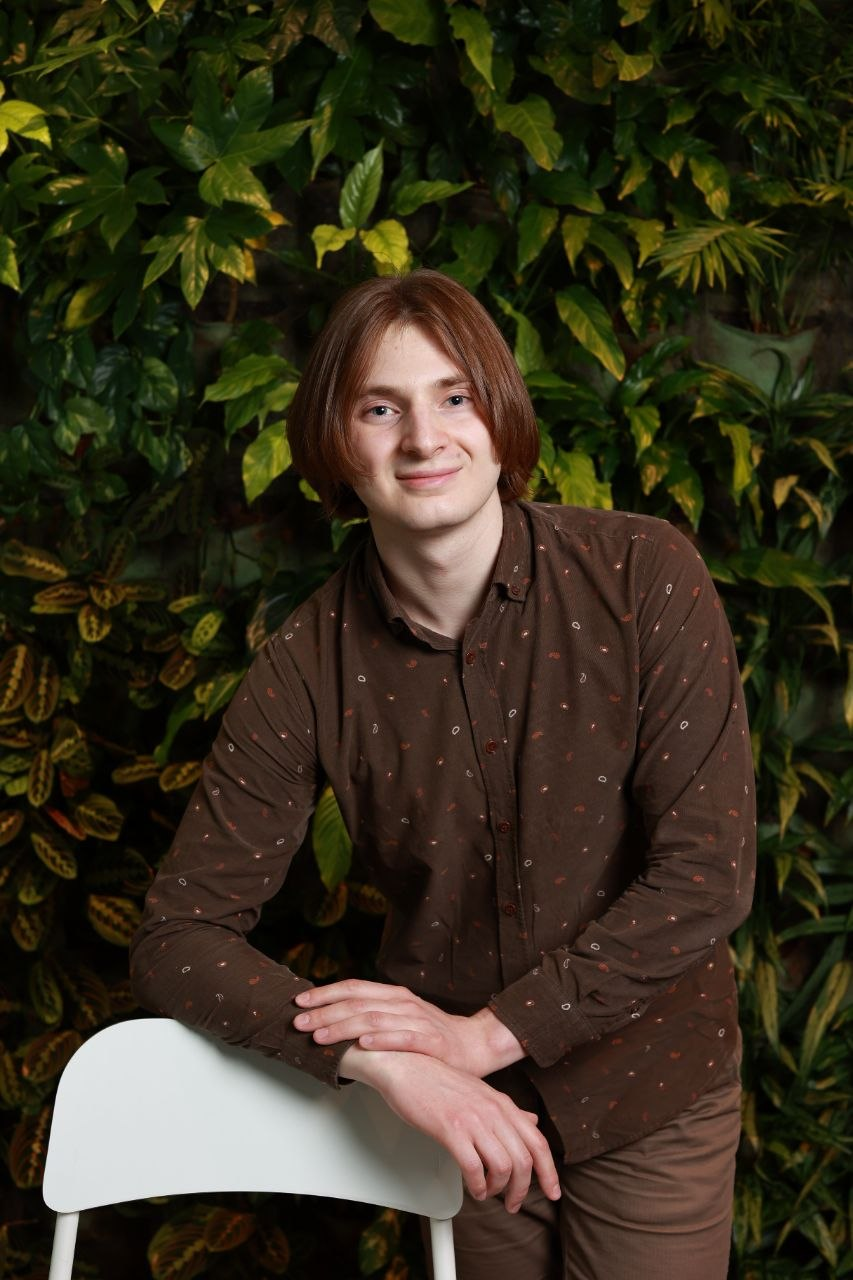
\includegraphics[width=1in,height=1.25in,clip,keepaspectratio]{images/authors/AlexanderKharitonov.jpg}}]{A. Kharitonov} holds a Master’s degree in Data Science from the Skolkovo Institute of Science and Technology. He began his career at Huawei, working pretraining and distillation of Large Language Models. He currently works at SberAI, focusing on the evaluation and validation of AI algorithms. His interests include model evaluation, trustworthy AI, and deploying machine learning benchmarks.
\end{IEEEbiography}

\vspace*{-15mm}

\begin{IEEEbiography}[{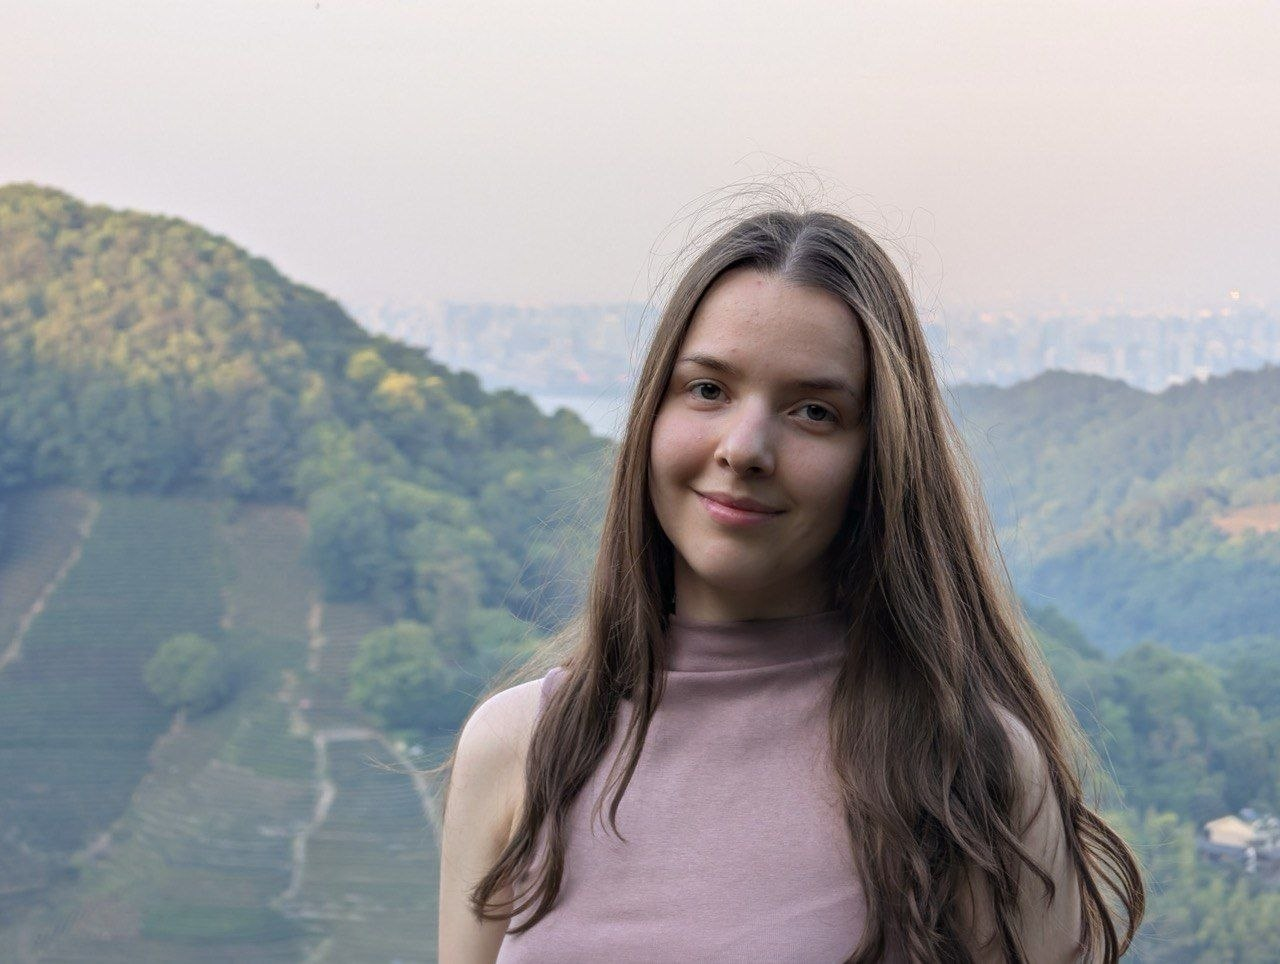
\includegraphics[width=1in,height=1.25in,clip,keepaspectratio]{images/authors/AlinaBogdanova.jpg}}]{A. Bogdanova} is a researcher specializing in large language model quantization at Huawei. She earned her bachelor’s degree in Mathematics from the Higher School of Economics. She later obtained a master’s degree in Data Science from Skolkovo Institute of Science and Technology (Skoltech). Her current work centers on improving the efficiency and deployment of large language models through quantization techniques, enabling faster and more resource-efficient AI systems. Her research interests include deep learning optimization, model compression, and scalable artificial intelligence systems.
\end{IEEEbiography}

% \vspace*{-15mm}

% \begin{IEEEbiography}[{\includegraphics[width=1in,height=1.25in,clip,keepaspectratio]{images/authors/MikhailBelkin.jpg}}]{M. Belkin} 
% \end{IEEEbiography}

\vspace*{-15mm}

\begin{IEEEbiography}[{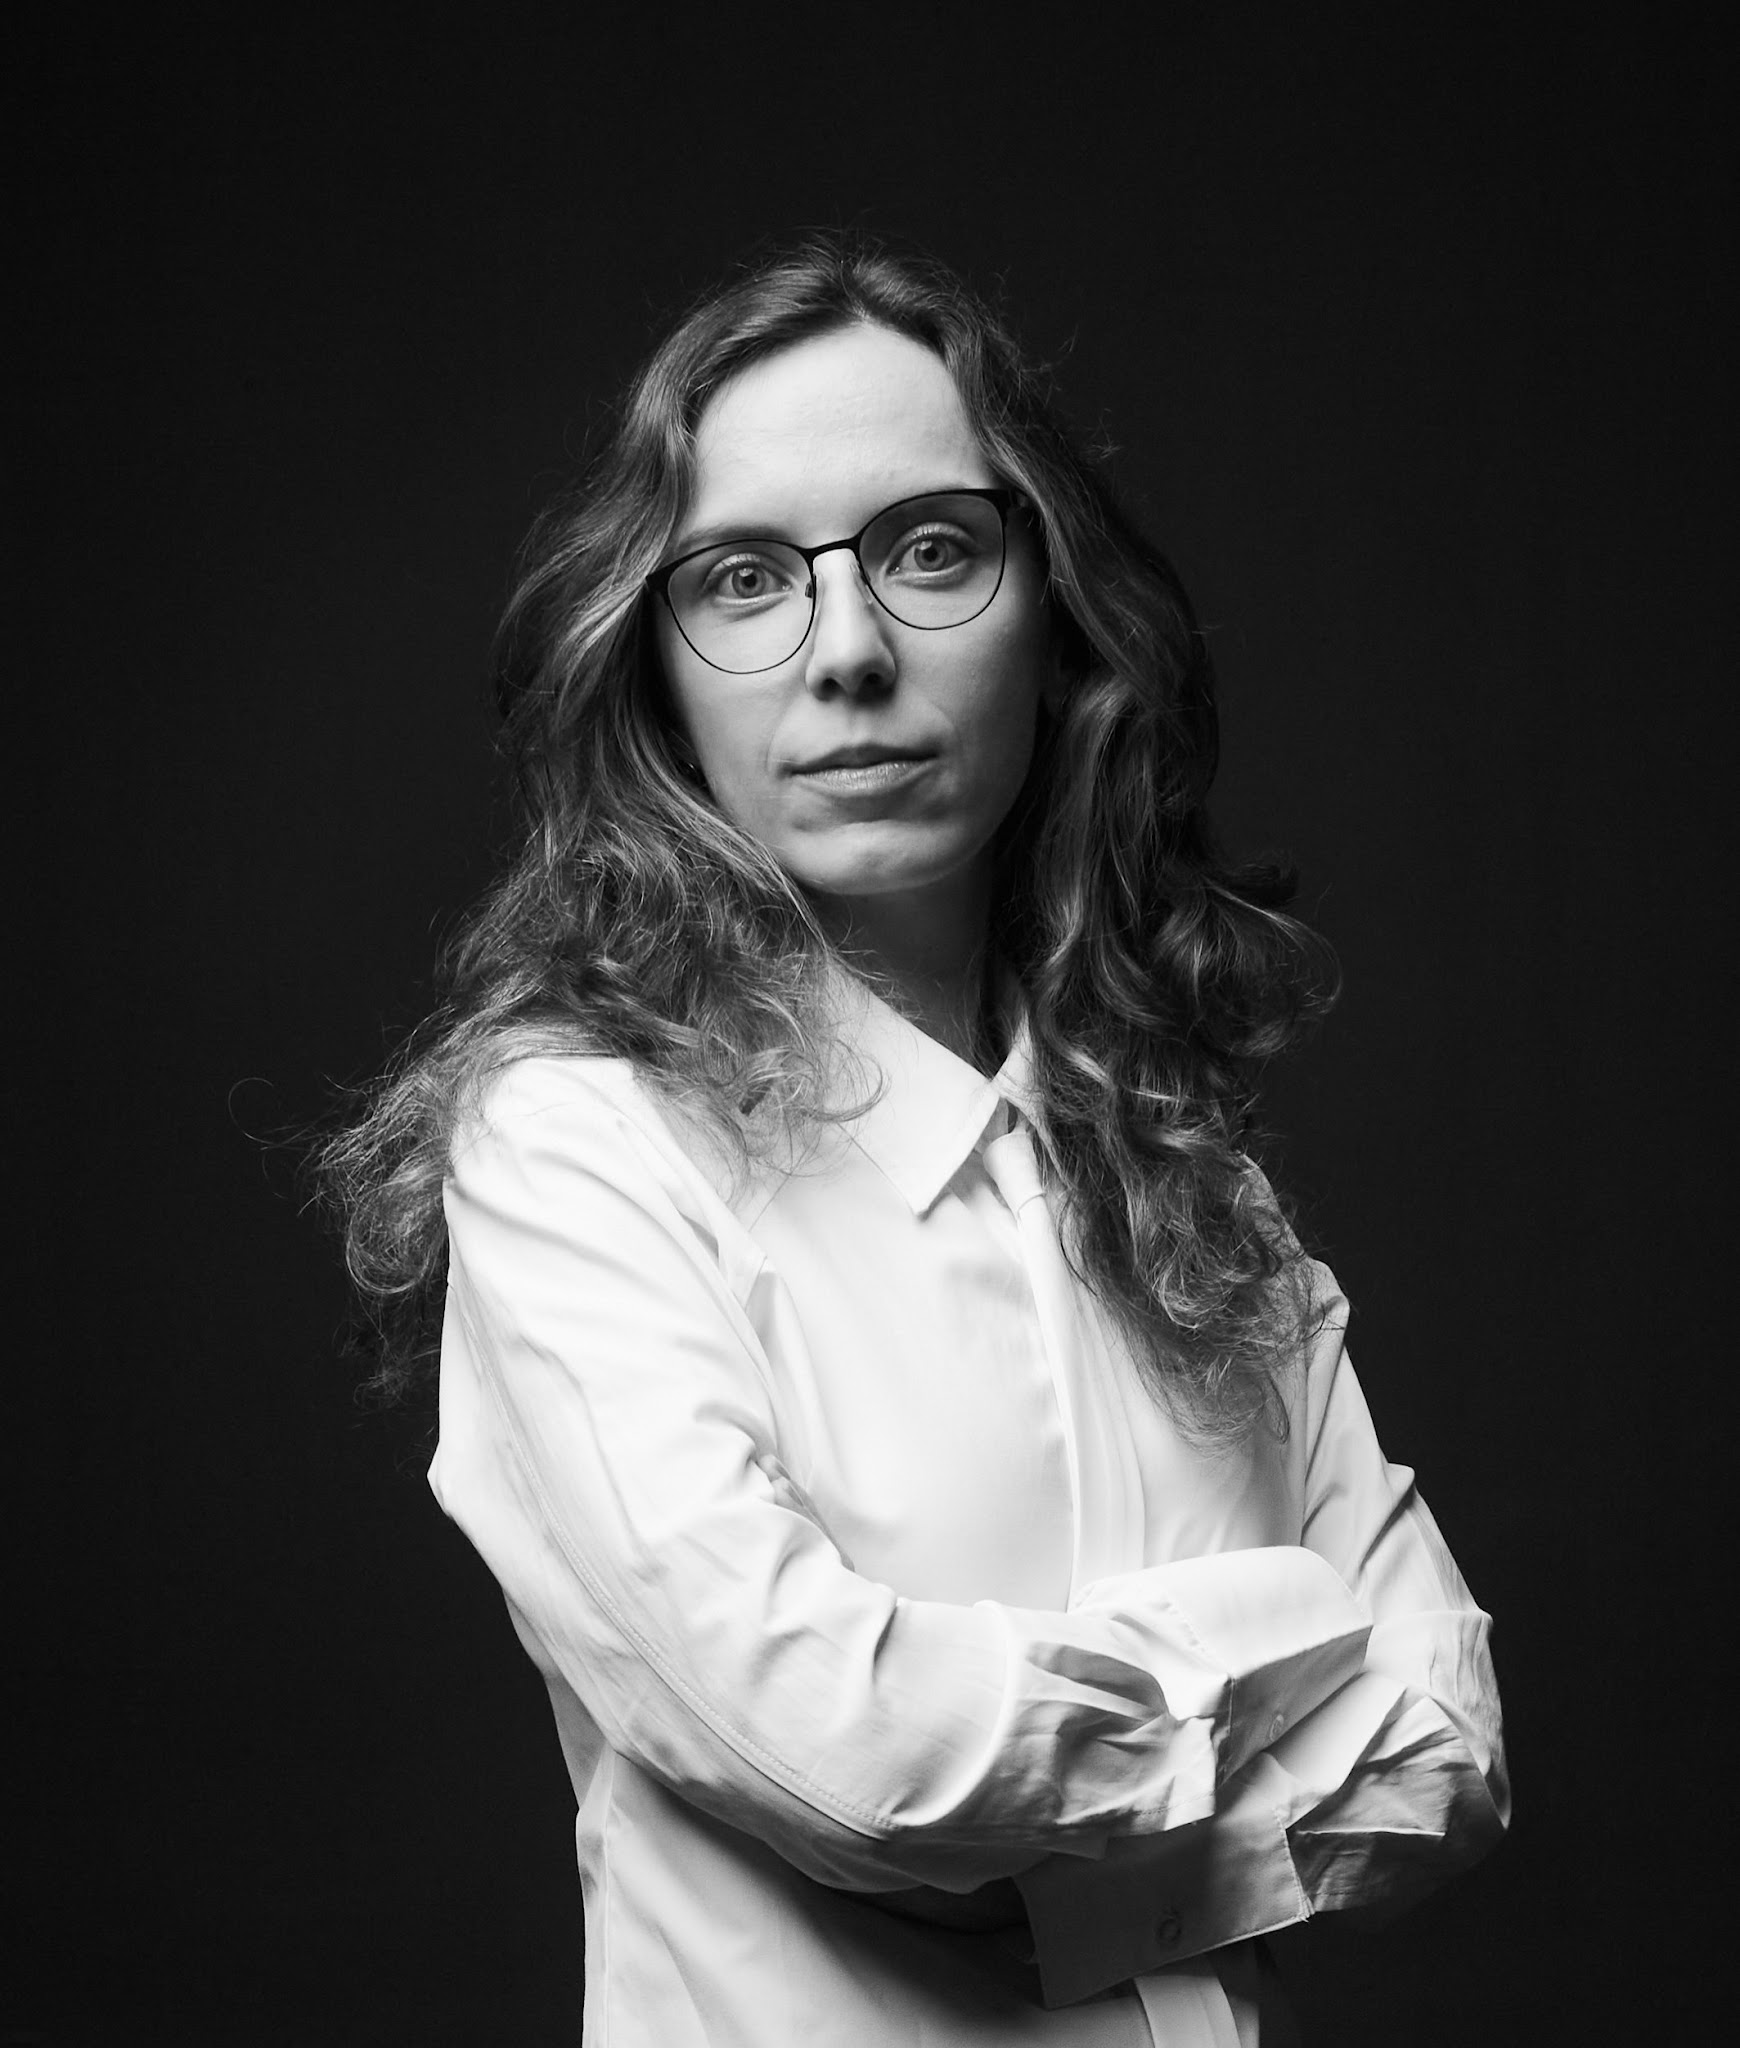
\includegraphics[width=1in,height=1.25in,clip,keepaspectratio]{images/authors/EkaterinaLisitsyna.jpg}}]{E. Lisitsyna} is a Lead Data Scientist at Sber. Graduated from the Computer Linguistics program at the Higher School of Economics (2020). Currently working on building AI models and agents for speech analytics and knowledge extraction from communications with corporate clients. The created AI solutions help to increase call-to-deal conversion for sales, as well as to automate the quality control of services and support provided by the corporate call center.
\end{IEEEbiography}

% \vspace*{-15mm}

% \begin{IEEEbiography}[{\includegraphics[width=1in,height=1.25in,clip,keepaspectratio]{images/authors/ArtemSosedka.jpg}}]{A. Sosedka} 
% \end{IEEEbiography}

\vspace*{-15mm}

\begin{IEEEbiography}[{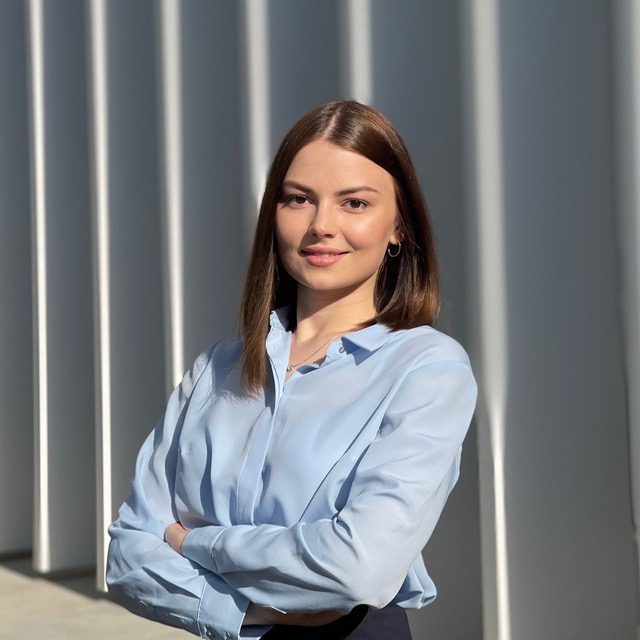
\includegraphics[width=1in,height=1.25in,clip,keepaspectratio]{images/authors/VictoriaDochkina.jpeg}}]{V. Dochkina} is the Director of the AI and Data Center, Strategy and Development Block, Sber. She leads the block’s strategic AI implementation and digital transformation initiatives.
Education: Bachelor’s and Master’s degrees with honors from the Moscow Institute of Physics and Technology (MIPT); Master’s degree from Skoltech, recipient of the 2021 Best Thesis Award; ongoing PhD at MIPT focused on multiagent AI systems and foundation model architectures.
Expertise: Development and deployment of enterprise-scale AI solutions; AI governance frameworks; Agentic AI.
Research interests: Foundation models; multimodal expansion; agentic LLM capability development; scaling AI agents for process automation; autonomous AI systems; mixture-of-experts architectures; coordination frameworks for enterprise-wide autonomization.
\end{IEEEbiography}

\vspace*{-15mm}

\begin{IEEEbiography}[{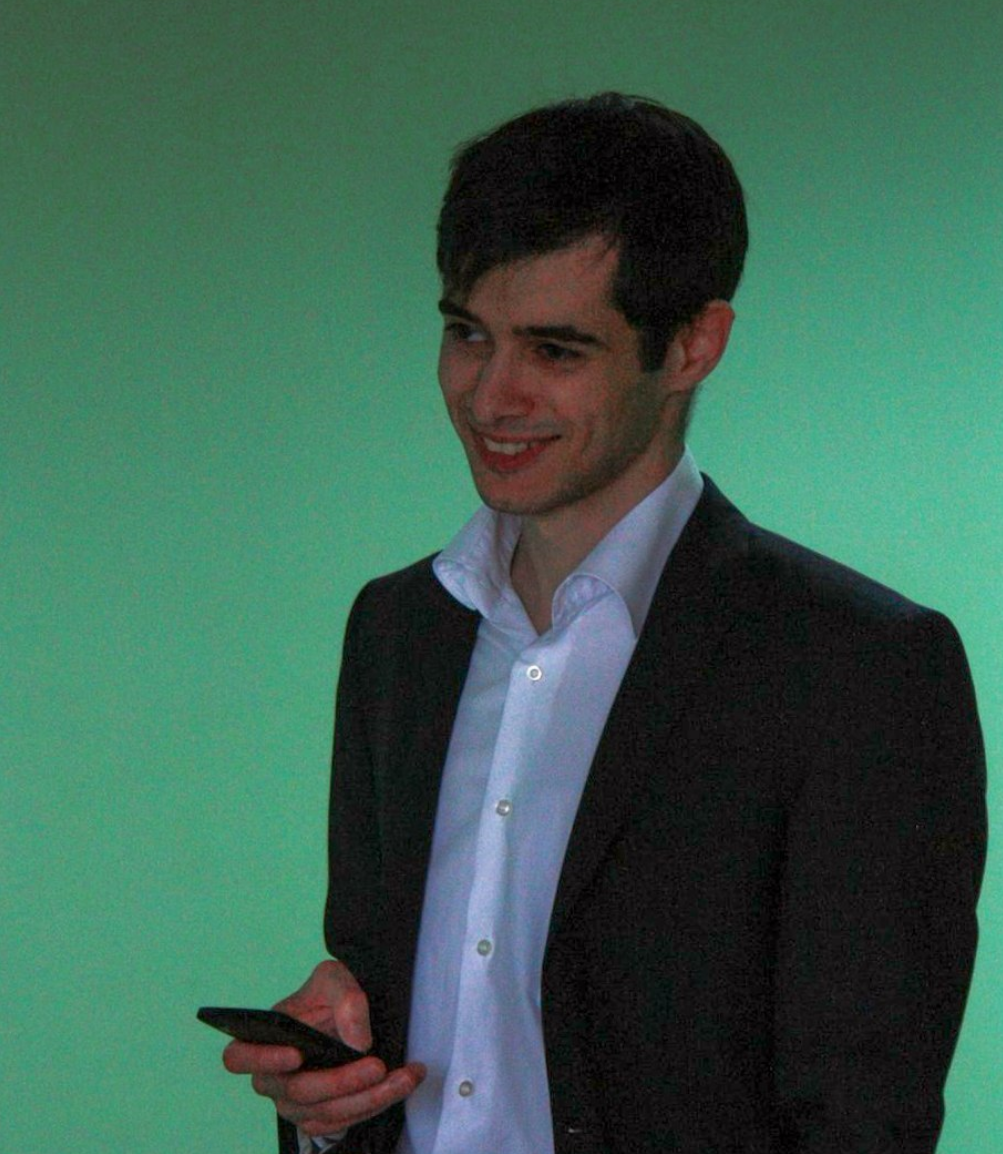
\includegraphics[width=1in,height=1.25in,clip,keepaspectratio]{images/authors/RuslanKostoev.png}}]{R. Kostoev} got M.Sc. degree in applied mathematics and computer science from Lomonosov Moscow State University, and built an impressive career spanning technology, innovation, and leadership roles. His professional journey includes experience at major companies such as Philips and Google, where he contributed to significant projects and initiatives. 
\end{IEEEbiography}

\vspace*{-15mm}

\begin{IEEEbiography}[{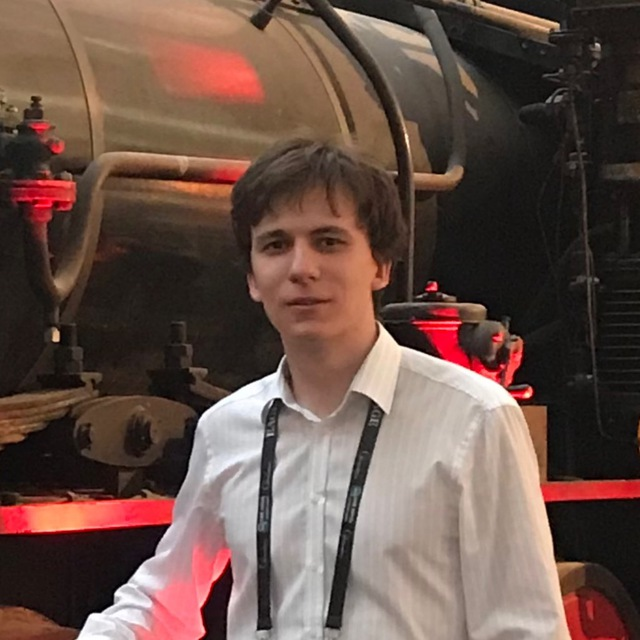
\includegraphics[width=1in,height=1.25in,clip,keepaspectratio]{images/authors/IliaPerepechkin.png}}]{I. Perepechkin} got M.Sc. degree in Applied Mathematics and Physics from Moscow Institute of Physics and Technology in 2017. He has experience developing enterprise-level AI solutions. He is currently a team lead data scientist at Sberbank, developing multi-agent systems.
\end{IEEEbiography}

\vspace*{-15mm}

\begin{IEEEbiography}[{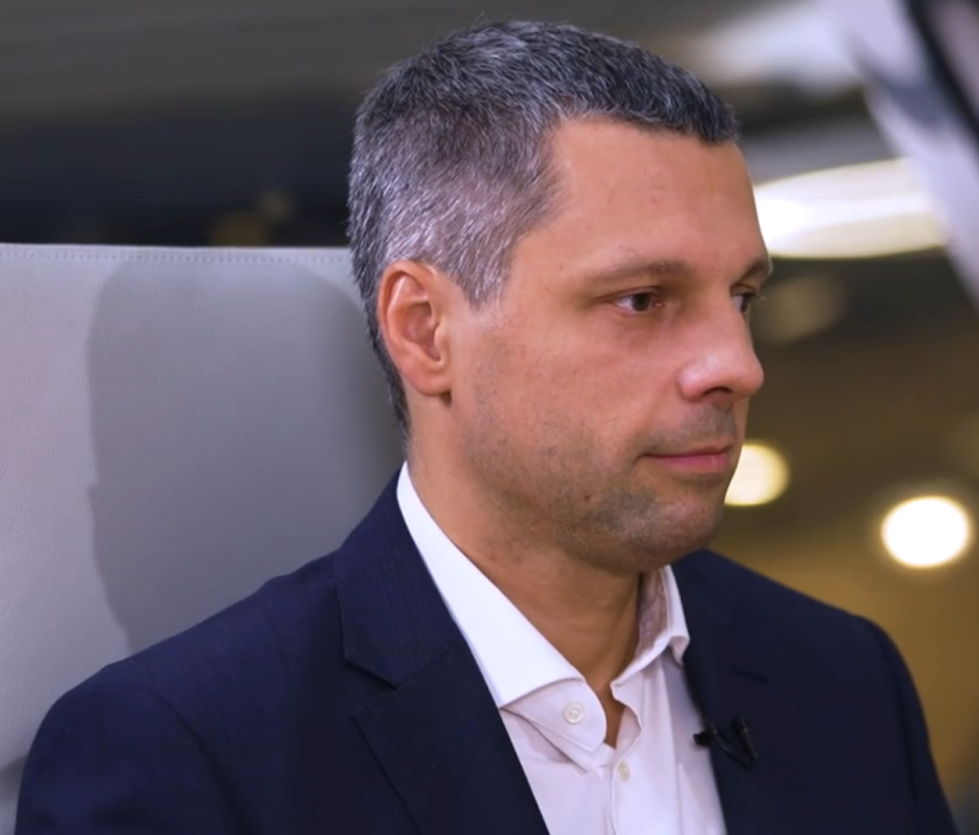
\includegraphics[width=1in,height=1.25in,clip,keepaspectratio]{images/authors/EvgenyBurnaev.png}}]{E. Burnaev} received the M.Sc. degree in applied physics and mathematics from Moscow Institute of Physics and Technology, in 2006, the Ph.D. degree in foundations of computer science from the Institute for Information Transmission Problem RAS, in 2008, and the Dr.Sci. degree in mathematical modeling and numerical methods from Moscow Institute of Physics and Technology, in 2022. 
He is currently the Director of the AI Center, Skolkovo Institute of Science and Technology, and a Full Professor. His research interests include generative modeling, manifold learning, deep learning for 3D data analysis, multi-agent systems, and industrial applications.
\end{IEEEbiography}
